\section{Theorie}
\label{sec:Theorie}

\subsection{Die Natur des Lichts}

Der Photoeffekt zeigt, dass die Wellenbeschreibung unzureichend ist, um alle Eigenschaften des Lichts
zu erklären. 
Für die Phänomene der Wechselwirkung des Lichtes mit Materie ist die Einführung des Photons als
Lichtteilchen notwendig. Erst wenn über viele Photonen gemittelt werden kann, findet die
Wellenbeschreibung wie beispielsweise bei Beugungsphänomenen wieder Verwendung.

\subsection{Der Photoeffekt}

Als Photoeffekt benannt ist die Herauslösung von Elektronen aus Metalloberflächen bei
(monochromatischer) Lichteinstrahlung. Die Energie des Lichtes, bzw. der sich mit der 
Lichtgeschwindigkeit $c$ linear ausbreitenden Photonen, ist als

\begin{equation}
    E_\lambda = h f \;
    \label{eqn:lichtenergie}
\end{equation}

gegeben, wobei $f$ die Lichtfrequenz beschreibt und $h$ das Plancksche Wirkungsquantum darstellt.

Die Energie, die ein Photon auf ein Elektron im Metall überträgt, wird aufgewendet, um die Austrittsarbeit
$W_\text{A}$ zur Heruslösung des Elektrons zu leisten. Die restliche Energie wird zur kinetischen Energie
$E_\text{kin,e}$ des Elektrons. Es ergibt sich:

\begin{align}
    E_\lambda &= h f = E_\text{kin,e} + W_\text{A} = \frac{1}{2} m_\text{e} v^2 \\
    \iff  E_\text{kin,e} &= h f - W_\text{A}  \; .
    \label{eqn:energie}
\end{align}

$E_\text{kin,e}$ wird also durch eine von $f$ abhängige Gerade beschrieben. Für den Bereich

\begin{equation*}
    h f < W_\text{A} = h f_\text{grenz}
\end{equation*}

kleiner der Grenzfrequenz $f_\text{grenz}$ tritt der Photoeffekt nicht auf, da die Austrittsarbeit $W_\text{A}$
nicht geleistet werden kann. 
Die Herauslösung der Elektronen ist entgegen der Wellentheorie abhängig von der Frequenz und nicht
von der Lichtintensität.

\subsection{Die experimentelle Untersuchung}

In Abbildung \ref{fig:bild1} sind links der Aufbau der Photozelle und rechts der gesamte Versuchsaufbau abgebildet.

\begin{figure}
    \centering
    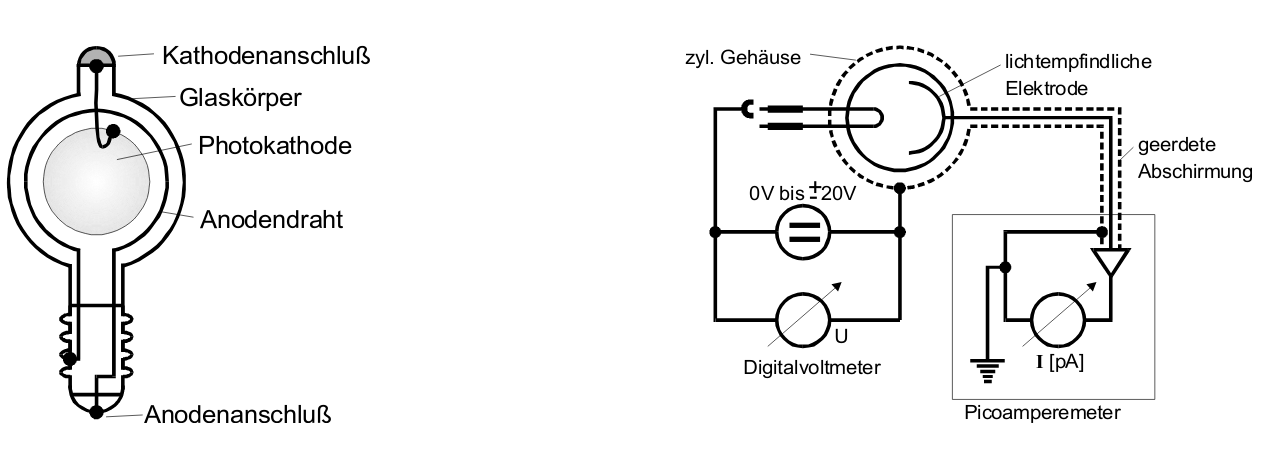
\includegraphics[scale=0.37]{content/bild1.png}
    \caption{Der Aufbau einer Photozelle (links) und der Versuchsaufbau (rechts). [1]}
    \label{fig:bild1}
\end{figure}

  Die kinetische Energie

\begin{equation}
    E_\text{kin,e} = \frac{1}{2} m_\text{e} v^2 = e U
    \label{eqn:Ekin}
\end{equation}

  wird mithilfe der Gegenfeldmethode bestimmt. Mit der Gegenspannung $U_\text{g}$ wird zwischen
  den Elektroden ein elektrisches Feld aufgebaut, welches die Elektronen bremst.
  Die Gegenspannung wird erhöht, bis kein Photostrom mehr gemessen wird. Mithilfe der 
  eingestellten Grenzspannung $U_\text{grenz}$ wird $E_\text{kin,e}$ für Elektronen
  mit der maximalen Geschwindigkeit $v_\text{max}$ bestimmt.

  Somit ergibt sich für Lichtenergie:

\begin{equation}
    E_\lambda = h f = e_0 U_\text{grenz} + W_\text{A} \; .
    \label{eqn:lichtenergie2}
\end{equation}

 Bei bekannter Lichtfrequenz lässt sich durch Umformung der Gleichung \eqref{eqn:lichtenergie2} die
 Austrittsarbeit $W_\text{A}$ bestimmen.

 Allerdings besitzen die herausgelösten Elektronen keinen diskreten Energiewert, sodass
 schon vorm Erreichen der Grenzspannung $U_\text{grenz}$ der Photostrom $I_\lambda$ merklich absinkt.
 Es ergibt sich der parabolische Zusammenhang 

 \begin{equation}
     I_\lambda(U) \sim U^2 \; ,
     \label{eqn:photostrom}
 \end{equation}

mit dem sich die Grenzfrequenz

\begin{equation}
    U_\text{grenz} = I_\lambda(0)
\end{equation}

bestimmen lässt.


  





